StreamStory is implemented as a client-server application, with its front-end implemented in HTML5,
CSS3 and JavaScript. The page layout is handled by Twitter Bootstrap 3, providing 
responsiveness and scalability to most modern devices. We use Cytoscape.js
for visualization of graphs and trees, including the main visualization, and D3.js for visualization of charts.
The front-end relies on technologies like Ajax and WebSockets for transparent real-time
updates.

The backend uses a hybrid implementation with its core functionality written in C++
as part of the QMiner data analytics platform \cite{qminer}, under the BSD license.
This functionality is exposed as a Node.js addon running in Googles V8 JavaScript
environment. Node.js thus acts as glue and exposes the functionality through RESTful
web services using the Express framework, also acting as the session manager.
User credentials \lstopar{and other information} are stored in a MySQL database.

Having the core functionality implemented in C++ provides performance benefits, especially
when dealing with larger datasets. When using StreamStory, the most time consuming step
is model initialization. Indeed, after this initial step, everything works in real-time.
The initialization includes partitioning the dataset, aggregating states, modeling transitions,
computation of state statistics, initialization of state assistance services and laying out the generated
hierarchical graph onto a plane. Our experiments show that the most time-consuming of these tasks are
the initialization of state assistance services, where a decision tree and a logistic regression
model need to be trained for each state in the hierarchical structure. State initialization tasks
are however independent and can be parallelized.

To measure the performance of the initialization procedure, we constructed several models on two datasets
of sizes 155MB (285k samples) and 500MB ($\approx$ \lstopar{3M} samples) respectively. A set of five attributes
was randomly chosen for each dataset and used in all the experiments. We
then constructed models with 18, 38 and 78 states respectively and measured the initialization times,
which we show in Figure \ref{fig:performance}.
\begin{figure}[h!]
	\centering
	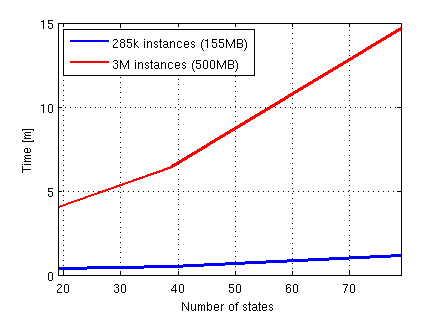
\includegraphics[width=0.7\columnwidth]{time-measurements}
	\caption{A graph of the measurements of the initial model construction time using two datasets, plotted against the number of states used for building the model.}
	\label{fig:performance}
\end{figure}
We can see that although the construction time increases with the number of states, the initialization
procedure is quite fast for the smaller data set with only the larger model with 78 states taking over 
a minute to complete. \lstopar{When using the larger dataset ...}

\lstopar{
\begin{itemize}
	\item the larger dataset was constructed in acceptable time
\end{itemize}
}

\iffalse
\begin{tabular}{ c | c c c c c}
	\label{tab:time-tests}
	 & 10 & 20 & 40 & reading CSV & file size \\
	\hline
	3229541 & 11min & 13min 32s & 21min 50s & 6:58,7:05,7:10 & 500MB \\
	285168 & 1:31 & 1:36 & 2:17 & 1:09,1:06,1:08 & 155MB
\end{tabular}
\fi